\subsubsection{GemNet}
\label{subsubsec:gemnet}

Gasteiger et al. $\!\!$ created GemNet (\enquote{Geometric Message Passing Neural Network}) 
\cite{https://doi.org/10.48550/arxiv.2106.08903} 
as an improvement over DimeNet and DimeNet++ (see 
\cite{DBLP:journals/corr/abs-2003-03123, https://doi.org/10.48550/arxiv.2011.14115} 
and \ref{subsubsec:dimenet}) that offers the flexibility for both energy-centric 
and force-centric predictions as well as 3-way or 4-way message passing.

Just like DimeNet and DimeNet++, GemNet 
takes the positions $\XX$ and atomic numbers $\zz$ of a molecule 
(defined in \eqref{eq:molecule_setup}) as inputs. For $a, b \in \set{1, \dots, n}$ write
\[
    d_{ab} \: \coloneqq \: \norm{\xx_b - \xx_a}_2 
    \qquad \text{and} \qquad 
    \vec{\xx}_{ab} \: \coloneqq \xx_b - \xx_a
\]
\begin{wrapfigure}{r}{0.3\textwidth}
    \centering
    \vspace*{-0.75em}
    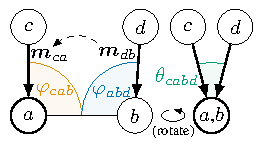
\includegraphics[]{atomic_simulations/gemnet_message_passing.pdf}
    \caption{\cite{https://doi.org/10.48550/arxiv.2106.08903}}
    \label{fig:gemnet-mp}
\end{wrapfigure}
for the distance and relative direction from $\xx_a$ to $\xx_b$ respectively.
In GemNet, there are two graphs considered: an interaction graph and an embedding graph.
The molecule's interaction graph does not change during the forward pass of the network and 
two atoms \textit{interact} if their distance is below some 
cutoff $c_{\text{int}}$. In addition to this interaction graph, all atom pairs 
whose distance is below some threshold $c_{\text{emb}}$ are \textit{embedded}---and, thus, 
edges of the embedding graph.

In contrast to DimeNet, the 3- or 4-way interactions for message passing are now used 
in a slightly different way:
Consider pairwise different $a, b, c, d \in \set{1, \dots, n}$,
where $(\_, a, b)$ are interacting and $(\_, c, a)$, $(\_, d, b)$ are
embedded. Set
\[
    \varphi_{cab} \: \coloneqq \: 
    \measuredangle \left( \vec{\xx}_{ca}, \vec{\xx}_{ab} \right)
    \qquad \text{and} \qquad
    \varphi_{abd} \: \coloneqq \: 
    \measuredangle \left( \vec{\xx}_{ab}, \vec{\xx}_{db} \right) \text{,}
\]
as well as 
\[
    \phi_{cabd} \: \coloneqq \: 
    \measuredangle \left( \boldsymbol{\Pi} \vec{\xx}_{ca}, \boldsymbol{\Pi} \vec{\xx}_{db} \right),
    \qquad \boldsymbol{\Pi} \: \coloneqq \: 
    \boldsymbol{I}_3 - \vec{\xx}_{ab} \vec{\xx}_{ab}^\top \text{,}
\]
where $\boldsymbol{\Pi}$ is the orthogonal projection on the orthogonal
complement of $\vec{\xx}_{ab}$ (see Figure~\ref{fig:gemnet-mp}).

Similarly to DimeNet, this relative directional information is then encoded by the
transformations
\[
    \eee_{\text{RBF}}^{(ca)} \: = \: \eee_{\text{RBF}}(d_{ca}), 
    \quad \eee_{\text{CBF}}^{(cab)} \: = \: \eee_{\text{CBF}}(d_{ca}, \varphi_{cab}),
    \quad \eee_{\text{SBF}}^{(cabd)} \: = \: \eee_{\text{SBF}}(d_{ca}, \varphi_{cab}, \phi_{cabd}) 
\]
which are related to DFT calculations.
These three quantity types $\eee_{\text{RBF}}^{(ca)}$, $\eee_{\text{CBF}}^{(cab)}$, $\eee_{\text{SBF}}^{(cabd)}$ 
can now be regarded as the (constant) features of the
molecule that are used by GemNet for updating the input graph.
In GemNet, the higher-order interactions are
\begin{align}
    T \: &\coloneqq \quad 
    \setcomp{(\_, c, a, b)}{c, a, b \in \set{1, \dots, n}, 
    \: d_{ca} \leq c_{\text{emb}}, \: d_{ab} \leq c_{\text{int}}} \label{eq:gemnet-triplets} \\
    &\qquad \cup  \setcomp{(\_, c, a, b, d)}{c, a, b, d \in \set{1, \dots, n}, 
    \: d_{ca} \leq c_{\text{emb}}, \: d_{ab} \leq c_{\text{int}}, 
    \: d_{db} \leq c_{\text{emb}}}; \label{eq:gemnet-quadruplets}
\end{align}
where the higher-order attributes are indexed by the involved nodes (contrary 
to the definition in \eqref{eq:higher_order_interact}), and all appearing $a, b, c, d$ 
are assumed to be pairwise different.

GemNet admits the following variants:
\begin{itemize}
    \item \textit{GemNet-T} is an energy-centric variant of GemNet that only uses the 3-way 
          interactions from \eqref{eq:gemnet-triplets}, which are updated 
          using $\eee_{\text{RBF}}^{(ca)}$ and $\eee_{\text{CBF}}^{(cab)}$.
          In Figure~\ref{fig:gemnet}, this is indicated by the 
          \textbf{\textcolor{tum-orange}{T}-MP} block.
    \item In contrast, \textit{GemNet-Q} is an energy-centric version of GemNet
          that also successively updates the 4-way interactions \eqref{eq:gemnet-quadruplets},
          taking the entirety of $\eee_{\text{RBF}}^{(ca)}$, $\eee_{\text{CBF}}^{(cab)}$
          and $\eee_{\text{SBF}}^{(cabd)}$ into account. In Figure~\ref{fig:gemnet}, this 
          is represented by the \textbf{\textcolor{tum-green}{Q}-MP} block.
\end{itemize}
Force-centric versions of GemNet-T and GemNet-Q are called \textit{GemNet-dT}
and \textit{GemNet-dQ} respectively.

\begin{figure}[H]
    \centering
    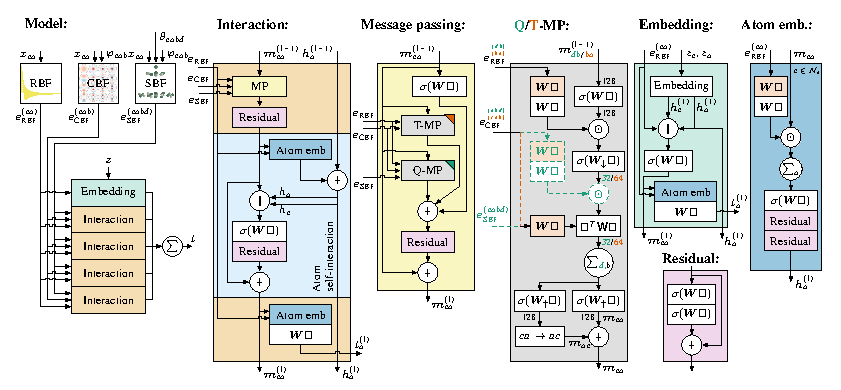
\includegraphics[]{atomic_simulations/gemnet.pdf}
    \caption{Complete architecture of GemNet as depicted in 
    \cite[Appendix F]{https://doi.org/10.48550/arxiv.2106.08903}.}
    \label{fig:gemnet}
\end{figure}
